\chapter{A finite element method for the Landau-Lifshitz-Gilbert Equation}
\label{sec:galerk-meth-llg}

In \cref{sec:intr-finite-ele-diff} we give a general introduction to the finite element method as applied to the magnetostatic potential equation \cref{eq:Hms} in one spatial dimension.
Then in \cref{sec:llg-initial-equations,sec:time-discretisation-resi} we extend this discussion to the full (non-linear) Landau-Lifshitz-Gilbert equation with magnetostatics in three spatial dimensions.
The linearisation of the LLG equation is handled using the Newton-Raphson method (see \cref{sec:newt-raph}), hence we need to derive an analytical expression for the Jacobian matrix.
This is done in \cref{sec:llg-jacobian-calculation}.

Finally in \cref{sec:nodal-integration} we show how the geometric integration properties of IMR (as discussed in \cref{sec:time-discretisation}) can be extended from the simple ODE case to the semi-discretised FEM.

For the purposes of \thisref{sec:galerk-meth-llg} we will assume that suitable boundary conditions on the magnetostatic potential have been already been determined, the details of this process are discussed in \cref{sec:hybr-finit-elem}.

\section{Introduction to the finite element method}
\label{sec:intr-finite-ele-diff}

The following simple problem is used to illustrate the finite element method:
Find $\phim(x)\in C^{2}(0,1)$ \footnote{The set $C^n(\magd)$ is the set of all functions $f$ such that $f$ and it's first $n$ derivatives are continuous on $\magd$.} such that
\begin{equation}
  -\phim''(x) = f(x) \qquad x \in (0,1),
  \label{eq:poisson1}
\end{equation}
with boundary conditions
\begin{equation}
  \phim(0)=\phim_{a},\quad \phim(1)=\phim_{b},\quad f=f(x)\in C(0,1).
\end{equation}
A function $g$ is in $C^{k}(\magd)$ if $g$ and it's first $k$ derivatives are continuous in $\magd$.
Setting $f = -\div \mv = -\pd{m_x}{x}$ results in the magnetostatic potential problem \cref{eq:Hms} with Dirichlet boundary conditions.

Before we can continue we need some definitions:
The function space $L^{2}$ consists of all functions $f$ such that $\sqrt{\int_{-\infty}^{\infty}\abs{f(x)}^{2} \d x}$ is finite.
The $n$-th Sobolev space, $\sob^n$, is the space of all functions $f$ such that $f$ and its first $n$ derivatives (with respect to all combinations of directions) are in $L^2$, \eg
\begin{equation}
  \label{eq:H1}
  \sob^1(\magd) = \setst{ \phim : [0,1] \rightarrow \mathbb{R} }{ \phim, \pd{\phim}{x_i} \in L^2(\magd) \; \forall x_i }
\end{equation}


\subsection{A weak formulation}
\label{Derivation-of-weighted-residuals}

The method of weighted residuals is the first step in a variety of modelling methods including the finite element method and the spectral method.
It involves replacing the initial PDE with an equivalent but more flexible version.

The formulation of the problem in \cref{eq:poisson1} (called a strong or classical formulation) is too restrictive for our purposes.
It disallows some useful approximating functions and restricts the geometries that can be modelled \cite[14]{HowardElmanDavidSilvester2006}.
For ``well behaved'' functions and domains a \emph{weak formulation} is equivalent but without these restrictions.
The weak formulation of \cref{eq:poisson1} is: find $\phim\in V_{s}$ such that
\begin{equation}
  -\intui{\phim'' v} = \intui{f v} \qquad \forall v \in V_{T},
  \label{eq:26}
\end{equation}
where $V_{T}$ is some appropriate space of \emph{test functions} and $V_{T}\subseteq \sob^0(0,1)$ in order to ensure that the integrals in \cref{eq:26} are well defined.
Additionally we do not need to enforce the boundary values in this way since they are known, so we can set the test functions to zero on the boundaries (this property is useful later on).
So an appropriate test function space is
\begin{equation}
  \label{eq:28}
  \begin{aligned}
    V_{T} &= \sob^0(0,1) \cap \Dfs_0, \\
    \Dfs_0 &= \setst{v}{v \in L^2(0,1),\; v(0) =0,\; v(1)=0}.
  \end{aligned} 
\end{equation}
The space $V_{s}$ is the solution space
\begin{equation}
  \begin{aligned}
    V_{s} &= \sob^2(0,1) \cap \Dfs, \\
    \Dfs &= \setst{\phim}{\phim \in L^2(0,1),\, \phim(0) = \phim_{a},\, \phim(1) = \phim_{b}},
  \end{aligned} 
\end{equation}
\ie the space of functions that are sufficiently smooth for the integrals to be finite and that satisfy the boundary conditions.

To see that \cref{eq:26} is equivalent to \cref{eq:poisson1} consider the case when $f(x) + \phim''(x)$ is non-zero at a point $x \in (0,1)$, \ie when the strong form \cref{eq:poisson1} is not satisfied. 
Since \cref{eq:26} must hold for all functions we can choose a function which is non-zero at $x$ and \cref{eq:26} will fail.
We call this approach the method of weighted residuals \cite[210, 214]{Zeinkiewicz1967}.

The smoothness restrictions on our weak form approximation can be further reduced by integrating the left hand side of \cref{eq:26} by parts to obtain
\begin{equation}
  -\intui{ \phim''v } = -\Big[ \phim'v \Big]_{0}^{1} + \intui{ \phim'v' } = \intui{f v}.
  \label{eq:29}
\end{equation}
Note that the square bracketed term in \cref{eq:29} is zero because the test functions, $v$, are set to zero on the boundary.
Hence we are left with the problem: Find $\phim \in \sob^1(0,1) \cap \Dfs$ such that
\begin{equation}
  \intui{ \phim'v' } = \intui{ fv } \quad \forall v \in \sob^1(0,1) \cap \Dfs_0.
  \label{eq:symmetric-weak-poisson}
\end{equation}
This rearrangement has removed the second derivative in $\phim$, hence we only require $\phim \in \sob^1(0,1)$ instead of $\phim \in \sob^2(0,1)$.
This allows a wider range of solution functions to be used, but comes at the expense of requiring more smoothness in the test functions.
It also means that our test and solution spaces are identical apart from the boundary values.

An alternative class of boundary condition, called Neumann conditions, specify the values of $\phim'$ at the boundary.
In this case we do not set the test functions to be zero on the boundary since the boundary values must still be determined as usual.
However knowing the value of $\phim'$ allows the bracketed term in \cref{eq:29} to be calculated directly.

\subsection{Discretisation}

\Cref{eq:symmetric-weak-poisson} is still continuous (\ie the test and solution spaces are still infinite dimensional) and so it cannot be implemented as a computational method.
To convert our continuous weak form to a discrete version we approximate the infinite dimensional test function space by a finite dimensional subset $V_{T}^{h} \subset \sob^1(0,1) \cap \Dfs$ such that
\begin{equation}
  V_{T}^{h} = \setst{v_h }{ v_h = \sum_{n=0}^{N}\alpha_{\ndi} \tbf_{\ndi},\, \alpha_{\ndi} \in \real} \cap \Dfs_0,
  \label{eq:30}
\end{equation}
for some finite set of test basis functions $\tbf_{\ndi}$.
Similarly, for $V_S^h \subset \sob^1(0,1) \cap \Dfs$:
\begin{equation}
  \label{eq:34}
  V_{S}^{h} = \setst{\phimh }{ \phimh = \sum_{l=0}^{N_l}\phim_{l} \sbf_{l},\, \phim_{l} \in \real}
  \cap \Dfs
\end{equation}
We call $\sbf_l$ the solution basis functions.
The distinction between the test functions, $\test$, and the test basis functions, $\tbf$, is often dropped because satisfying the weak form for all test basis functions implies that it is satisfied for all test functions.
Different choices of $\tbf_{\ndi}$ and $\sbf_l$ lead to different methods, the choice corresponding to the finite element method will be discussed in \cref{sub:Actual-Finite-Elements}.
For now we continue with a description of the conversion to a general discrete form.

Replacing $v_{h}$ from \cref{eq:poisson1} by $\tbf_{\ndi}$ gives an equivalent set of conditions
\begin{equation}
  \intui{  \phim'_{h} \tbf_{\ndi}'  }  = \intui{ f\tbf_{\ndi} } \qquad n=0,\ldots,N,
  \label{eq:discrete_weak_test_fns_replaced}
\end{equation}
Since $\phim_{h}\in V_{S}^{h}$ we can replace $\phim_{h}$ by a linear combination of the solution basis functions, \ie
\begin{equation}
  \phim_{h}=\sum_{l=0}^{N_l} \phim_{l}\sbf_{l},
  \label{eq:y-spans}
\end{equation}
where $\phim_l \in \real$ are the unknown coefficients which define the approximate solution $\phimh$.
Substituting \cref{eq:y-spans} into \cref{eq:discrete_weak_test_fns_replaced} gives
\begin{equation}
  \sum_{l=0}^{N_l} \phim_{l}\intui{ \sbf_{l}'\tbf'_{\ndi} } =\intui{ f\tbf_{\ndi} } 
  \qquad n=0,\ldots,N.
  \label{eq:31}
\end{equation}

The functions $f$, $\tbf$ and $\sbf$ are known and so the integrals in \cref{eq:31} can be evaluated.
Hence we introduce a matrix $\Am$ and a vector $\bv$ containing the results of these integrals:
\begin{equation}
  \begin{aligned}
    \Am_{l\ndi} &= \intui{ \sbf_{l}'\tbf'_{\ndi} }, \\
    b_{j} &= \intui{ f\tbf_{\ndi} }. \\
    \label{eq:Aij_bj}
  \end{aligned}
\end{equation}
and the problem is reduced to a system of linear equations.
Writing $\phimdis$ for the vector of $\phim_l$ the system is
\begin{equation}
  \Am \phimdis = \bv.
  \label{eq:final_galerkin}
\end{equation}
This system can be solved to find $\phimdis$, which can then be substituted into \cref{eq:y-spans} to give an approximation for $\phim(x)$.


\subsection{Finite Elements in One Dimension}
\label{sub:Actual-Finite-Elements}

To create a usable implementation of the methodology derived in so far in \thisref{sec:galerk-meth-llg} we must need to define basis functions for the spaces $V_{T}^{h}$ and $V_S^h$.
We choose the test and solution basis functions to be the same (except at the boundaries): $\sbf_l = \tbf_l$.
This choice defines a Galerkin method (and results in a symmetric matrix $\Am$ if the original equation has the corresponding symmetry) \cite[215]{Zeinkiewicz1967}.

The aim now is to approximate an arbitrary function by a linear combination of a finite set of easy-to-work-with functions, $\tbf_\ndi$.
A good class of functions to satisfy aim is the polynomials: they are trivial to add, subtract and differentiate; and can be easily numerically integrated (see \cref{sec:numer-eval-integrals}).

Additionally it is desirable that the final matrix $\Am$ be sparse (to allow efficient linear algebra).
For this to happen we need $\intui{ \sbf_{l}'\tbf'_{\ndi} } = 0$ for most pairs of $l, \ndi$. 
An obvious way to achieve this is to have each basis function only overlap (in space) with a few other basis functions, for example by having each basis function non-zero only on a portion of the domain.
Basis functions with this property are said to have ``local support''.

These two ideas lead us to the use of a carefully constructed set of \emph{piecewise polynomials} as our basis functions.
We first split the domain into $N_e$ non-overlapping regions called \emph{elements}, each with a \emph{node} at either end.
We then define two ``local'' basis functions within each element as
\begin{equation}
  \tbf^{(e)}_{0}=\dfrac{x-x^{(e)}_{1}}{x^{(e)}_{0}-x^{(e)}_{1}},\qquad
  \tbf^{(e)}_{1}=\dfrac{x-x^{(e)}_{0}}{x^{(e)}_{1}-x^{(e)}_{0}},
  \label{eq:simple_lagrange}
\end{equation}
where $x^{(e)}_0$ and $x^{(e)}_1$ are the positions of the nodes of element $e$.
This definition results in following useful properties of $\tbf^{(e)}_{\ndi}(x)$:
\begin{equation}
  \label{eq:35}
  \tbf^{(e)}_{\ndi}(x_{\ndi}) =
  \begin{cases}
    1 & k = \ndi, \\
    0 & k \neq \ndi.
  \end{cases}
\end{equation}
This means that the coefficient of each basis function in \cref{eq:y-spans} corresponds directly to the value of the solution at the node where that test function is non-zero
In other words the list of coefficients, $\phimdis$, is just a list of the nodal values of $\phim(x)$.

Next we define the $\ndi$th (global) basis function as:
\begin{equation}
  \label{eq:33}
  \tbf_\ndi(x) =
  \begin{cases}
    \tbf_\ndi^{(e)}(x) & \text{if $x \in [x^{(e)}_0, x^{(e)}_1]$ and node $\ndi$ is in element $e$,} \\
    0 & \text{otherwise.}
  \end{cases}
\end{equation}
So each global basis function is only non-zero on the elements neighbouring the node where it has a maximum value.
We call the set of such polynomial basis functions $\tsbasis$.
The relationship between the local and global test functions is illustrated in \cref{fig:local_global_functions}.  

\begin{figure}
  \center
  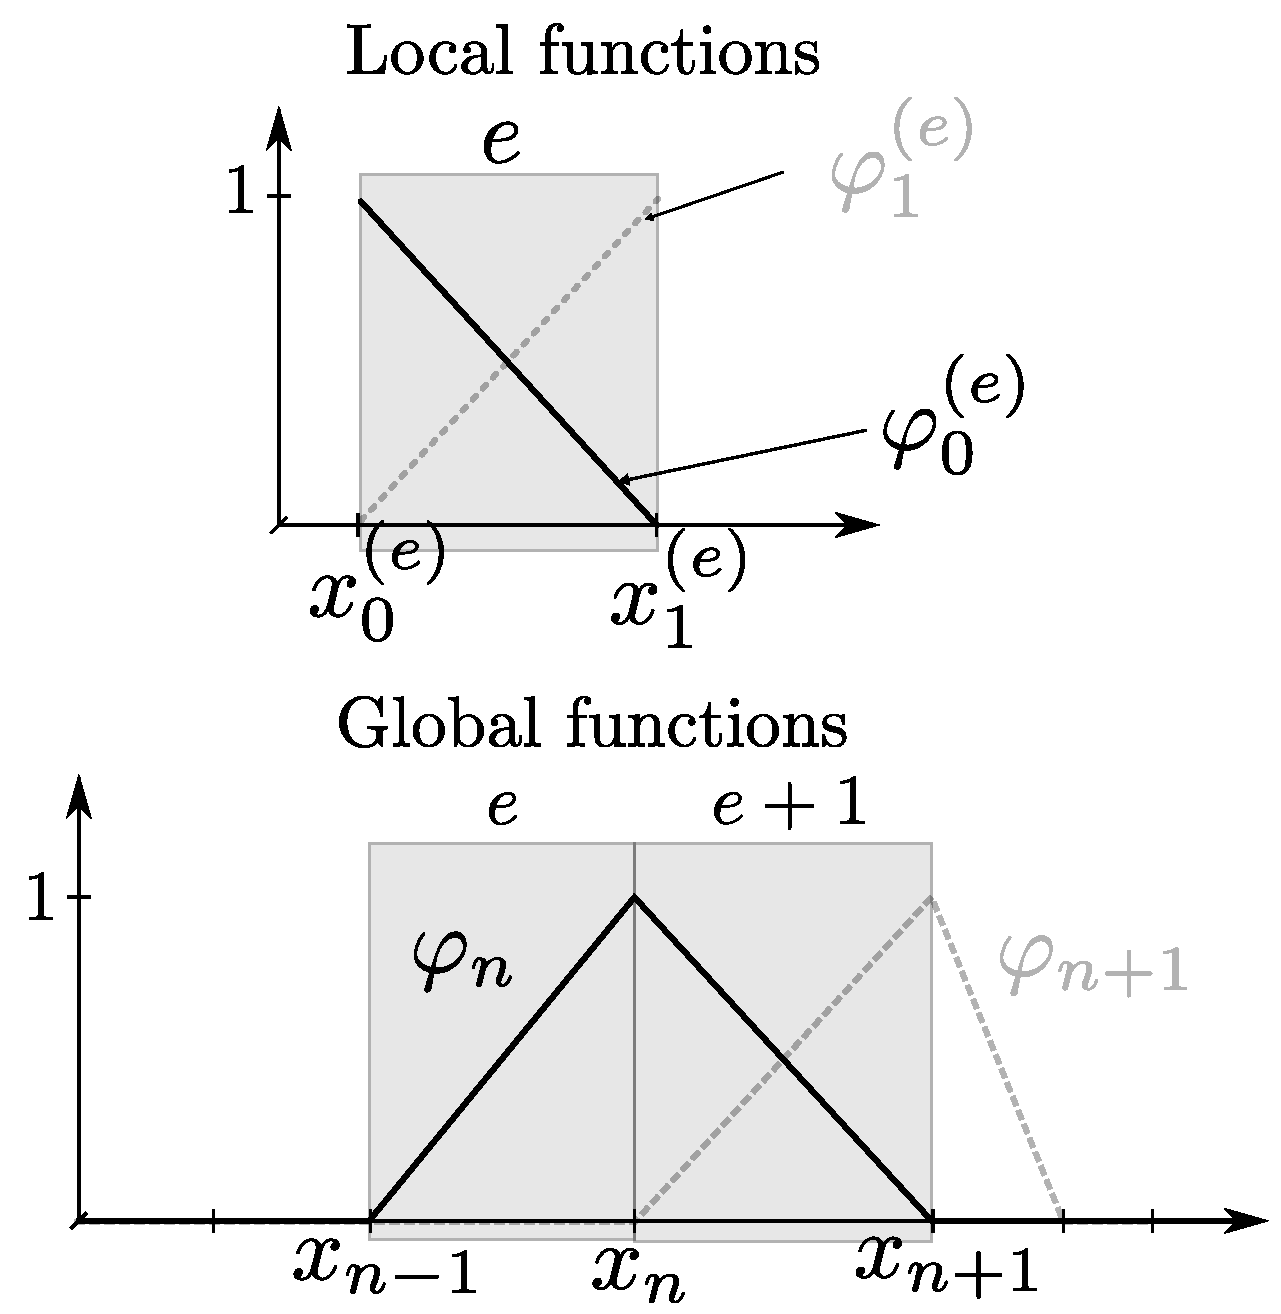
\includegraphics[width=0.8\textwidth]{./images/local_global_functions}
  \caption{The local and global piecewise polynomial basis functions and numbering schemes for a one-dimensional finite element model.  ??ds numbering: change $e_i$ to element $e$, $e_{i+1}$ to $e+1$, $x_i$ to $x_\ndi$, $x^(i)$ to $x^(e)$ $L_i$ to $\tbf_\ndi$
  }
  \label{fig:local_global_functions}
\end{figure}

The global basis functions are clearly in $\sob^1(0,1)$ since they are just piecewise polynomials.
So to obtain basis functions which satisfy the requirements on $V_T^h$ and $V_S^h$ we merely need to take the intersection with $\Dfs_0$ or $\Dfs$ respectively (\ie we discard the basis functions which do not obey the conditions on the boundary).

It is advantageous to work with such low order polynomials even for very complex models because the evaluation of integrals and interpolated values is simple and cheap to compute.
Also note that an arbitrary level of accuracy can be achieved when approximating a smooth function by piecewise polynomials by increasing the number of polynomials used (\ie by adding more nodes and elements to the mesh in appropriate places).

The description here generalises to higher dimensions fairly easily \cite[20]{HowardElmanDavidSilvester2006}.
In 2D square or triangle elements are typically used and nodes are placed at every corner of each element.
In 3D ``brick'' or tetrahedral elements are used in the same way.
In both cases the polynomial basis functions are replaced by higher dimensional ones with equivalent properties.

The method can also be generalised to higher order polynomials, although more nodes are required inside each element in order to provide enough values to fully define the polynomials.
The use of higher order polynomials increases the order of accuracy at the cost of speed: the resulting linear systems become more dense as the order of the polynomials is increased due to more basis functions overlapping with each other.

To calculate the matrix $\Am$ and the vector $\bv$ from \cref{eq:Aij_bj} we first calculate the local contributions from each element: $\Am^{(e)}$ and $\bv^{(e)}$.
We then assemble the global $\Am$ and $\bv$ by summing the appropriate local contributions.
For our one-dimensional Poisson example the calculation of $\Am^{(e)}$ is quite
simple: substituting the two local basis functions \cref{eq:simple_lagrange} into
\cref{eq:Aij_bj} and writing $h=x_{1}^{(e)} - x_{0}^{(e)}$ we are left with
\begin{equation}
  \Am^{(e)} = \frac{1}{h}
    \begin{pmatrix}
      1 & -1 \\
      -1 & 1
    \end{pmatrix},
\end{equation}
where $h$ is the element size, $h = x_{1}^{(e)}-x_{0}^{(e)}$ (note that $h$ can vary between elements).
Similarly for $\bv^{(e)}$ we obtain
\begin{equation}
  \bv^{(e)}=\frac{1}{h}
    \begin{pmatrix}
      -\int_{x_{0}^{(e)}}^{x_{1}^{(e)}}(x-x_{1}^{(e)})\, f(x)\, dx\\
      \int_{x_{0}^{(e)}}^{x_{1}^{(e)}}(x-x_{0}^{(e)})\, f(x)\, dx
    \end{pmatrix}
\end{equation}
which we compute numerically since the entries depend on $f(x)$.



\subsection{Numerical evaluation of integrals}
\label{sec:numer-eval-integrals}

In the above example the integrals for $\Am$ were fixed and so could be calculated analytically but this is not usually the case (\eg the vector $\bv$, or the Jacobian matrix for non-linear problems), so we need some method to evaluate the integrals computationally.
The most flexible way to evaluate integrals is numerically using a quadrature scheme.
A quadrature scheme is an approximation to an integral of the form
\begin{equation}
  \begin{aligned}
    \intdx{f(\xv)} &\approx  \sum_i w_i f(\xv_i),
  \end{aligned}
\end{equation}
where $\xv_i$ are the \emph{knots} (or evaluation points) and $w_i$ the weights.
The choice of $\xv_i$ and $w_i$ defines the quadrature scheme.

There exist many quadrature schemes suited for different applications.
Since we only need to evaluate integrals of polynomial functions a single simple and accurate class of quadrature is sufficient: Gaussian quadrature \cite[492]{Kincaid2002}.
Gaussian quadrature is able to exactly evaluate integrals of polynomials up to order $2n + 1$, the highest possible order, because the knots and weights are chosen to minimise the error for polynomial integration.

In higher dimensions the integration is not quite so simple.
Quadrature schemes only apply for integrals over specific shapes (or at they least must be non-trivially modified for alternative geometries).
To get around this issue we use a coordinate transformation to a reference element \cite[29]{HowardElmanDavidSilvester2006}, \eg any four sided element is mapped to the square $[-1, 1] \times [-1, 1]$, meaning that standard quadrature schemes can be used.
The final difficulty is then to calculate the Jacobian of this transformation: if the ``local'' position variable (\ie within the reference element) is $\sv$ then the Jacobian is
\begin{equation}
  J = \abs{ \pd{\sv}{\xv}} = \frac{1}{\abs{\pd{\xv}{\sv}}},
\end{equation}
where the elements of the Jacobian matrix $\pd{\xv}{\sv}$ can be calculated by interpolating $x$ using the local solution basis functions and differentiating.
When using linear polynomial basis functions the Jacobian is constant for 1D line elements, 2D triangular elements and 3D tetrahedral elements.

So the final integration scheme is
\begin{equation}
  \begin{aligned}
    \intdx[\magd_e]{f(\xv)} &= \intds[\magd_e]{f_s(\sv) J_e(\sv)}, \\
    &\approx  \sum_{i=0}^N w_i f_s(\sv_i) J_e(\sv_i).
  \end{aligned}
\end{equation}
where $f$ in terms of the local coordinate $\sv$ is
\begin{equation}
  f(\sv) = f\bigb{\sum_j \xv_j \sbf_j(\sv)}.
\end{equation}

Gaussian quadratures for square and cube elements can be trivially constructed from the one dimensional quadrature using a tensor product formula.
Similar ``full integration'' quadratures for triangular and tetrahedral elements exist \eg \cite{oomph-lib-integral.cc} ??ds cite actual papers.




\section{The FEM applied to the LLG equation}
\label{sec:llg-initial-equations}

We now apply the finite element method as discussed in \cref{sec:intr-finite-ele-diff} (together with the Newton-Raphson discussed in \cref{sec:newt-raph}) to the solution of the Landau-Lifshitz-Gilbert equation.
We use the Gilbert form of the LLG, \cref{eq:Gilbert}, with the effective fields described in \cref{sec:energy-magnetic-body} and the using potential method described in \cref{sec:magstat-field-calc-pote} for calculating the magnetostatic field.

We chose the Gilbert form of the LLG even though it is less intuitive because only contains single cross product terms, reducing the complexity of derivations.
A side effect of this choice is that explicit time integration schemes cannot be used since the time derivative is only defined implicitly.

\subsection{Initial equations}

After non-dimensionalisation (see \cref{sec:land-lifsh-gilb-normalisation}) the Landau-Lifshitz-Gilbert equation with effective field $\hv$ is given by
\begin{equation}
  \begin{aligned}
    \dmdt &= - \mv \times \hv + \alpha \mv \times \dmdt, \\
    \hv &= \happ - \grad \phim + \lap \mv + \kone (\mv \cdot \ev) \ev, \\
    \lap \phim &= \div \mv.
    \label{eqn:ndllg-starting}
  \end{aligned}
\end{equation}

For now we consider the magnetostatic potential only within the magnetic domain, $\magd$, with Neumann or Dirichlet boundary conditions on the boundary, $\boundd$.
Details of the extension to include the effects of the external region using the FEM/BEM method are given in \cref{sec:hybr-finit-elem}, for which both the Dirichlet and Neumann cases will be required.
We define $\boundd_\Dir$ and $\boundd_\Neu$ respectively to represent the region of the boundary domain where a Dirichlet condition or Neumann is imposed on the potential,\footnote{These must obviously be such that $\boundd_\Neu \cap \boundd_\Dir = \emptyset$ and $\boundd_\Neu \cup \boundd_\Dir = \boundd$.} \ie 
\begin{equation}
  \begin{aligned}
    \phim(\xv) &= g_\Dir(\xv) \quad \forall \xv \in \boundd_\Dir, \\
    \grad \phim(\xv) \cdot \nv(\xv) &= g_\Neu(\xv) \quad \forall \xv \in \boundd_\Neu,
  \end{aligned}
\end{equation}
where $\nv(\xv)$ is the outward unit normal.
We also define the following function spaces for convenience
\begin{equation}
\begin{aligned}
  \label{eq:037}
  \Dfs & = \setst{ v }{ v(\xv) = g_\Dir(\xv) \; \forall \xv \in \boundd_\Dir }, \\
  \Dfs_0 &= \setst{ v }{ v(\xv) = 0 \; \forall \xv \in \boundd_\Dir }.
\end{aligned}
\end{equation}

Recall from \cref{sec:magn-bound-cond} that the boundary condition on the magnetisation is
\begin{equation}
  \label{eq:m-bc}
  \mv \times \dmdn = \zerov \quad \forall \xv \in \boundd.
\end{equation}
It turns out that this Neumann-like condition is exactly what is needed in the derivation of the residuals.


\subsection{The weak form}
\label{sec:weak-form-residuals}

We now convert \cref{eqn:ndllg-starting} into the residual weak form as described in \cref{Derivation-of-weighted-residuals}.
In the following we will need the identity\footnote{This can be easily derived by applying the product rule to $\div (v \grad \phim)$.}
\begin{equation}
  (\lap \phim) \test = \div (v \grad \phim) - \grad \phim \cdot \grad v.
  \label{eq:20}
\end{equation}
We will also make use of the divergence theorem
\begin{equation}
  \intd{\div \fv} = \intb{\fv \cdot \nv}.
  \label{eq:div-thm}
\end{equation}

The Newton-Raphson residual for the magnetostatic potential is given by
\begin{gather}
  \rphi(\phim, \test) = \intd{ (\lap \phim) \test }
  - \intd{ (\div \mv) \test}, \label{eqn:phires1}
\end{gather}
where $\phim \in \sob^2(\magd) \cap \Dfs$ and $\mv \in \sob^1(\magd)$.

Recall that problem is to find some $\phim$ such that $\rphi(\phim, \test) = 0$ for all test functions $\test \in \sob^0(\magd) \cap \Dfs_0$.
We will find an approximation to $\phim$ using the Newton-Raphson method.
Note that while the use of a linearisation method is unnecessary for the magnetostatic potential alone (since \cref{eqn:phires1} is linear in $\phim$) it will be necessary for the overall problem.

We now reduce the order of the derivatives on $\phim$, as discussed in \cref{Derivation-of-weighted-residuals}, by ``transferring'' the derivatives onto the test functions.
Integrating identity \cref{eq:20} over the domain and applying the divergence theorem \cref{eq:div-thm} we obtain
\begin{equation}
  \begin{aligned}
    \intd{ (\lap \phim) \test} &=  \intd{\div (\test \grad \phim)}
           - \intd{\grad \phim \cdot \grad \test},\\
    &= \intb{\test (\grad \phim \cdot \nv)} 
    - \intd{ \grad \phim \cdot \grad \test}.
    \label{eqn:identitygauss}
  \end{aligned} 
\end{equation}
Substituting \cref{eqn:identitygauss} into \cref{eqn:phires1} gives
\begin{equation}
  \rphi(\phim, \test) = \intb{ \test (\grad \phim \cdot \nv) }
  - \intd{ \grad \test \cdot \grad \phim }
  - \intd{ (\div \mv) \test },
\end{equation}
where the function spaces are now $\phim \in \sob^1(\magd) \cap \Dfs$ and $v \in \sob^1(\magd) \cap \Dfs_0$.

Note that the boundary integral is always zero on $\boundd_\Dir$ by the definition of the test functions. 
Hence the boundary integral is only non-zero over $\boundd_{\Neu}$ where $\grad \phim \cdot \nv = g_{\Neu}$ and we have
\begin{equation}
  \rphi(\phim, \test) = \int_{\boundd_\Neu} \test g_\Neu \d \boundd
  - \intd{ \grad \test \cdot \grad \phim}
  - \intd{ (\div \mv) \test}.
  \label{res:contphi}
\end{equation}


Next we apply the same procedure to the Landau-Lifshitz-Gilbert equation with effective fields \cref{eqn:ndllg-starting}.
For now we sidestep the details of time discretisation by assuming $\dmdt$ to be just another (sufficiently smooth) function of $\xv$.
The weak form of the LLG is
\begin{equation}
  \begin{aligned}
    \rllgv(\mv, \test) = \int_\magd &\Big( \dmdt
    + (\mv \times \hca) + (\mv \times \happ) \\
    &- (\mv \times \grad \phi) + (\mv \times \lap \mv) - \dampc \left( \mv
      \times \dmdt \right) \Big) \test \d\magd. 
    \label{res:contllg}
  \end{aligned}
\end{equation}
Similarly to the previous examples the idea is to apply the Newton-Raphson method to find $\mv \in \sob^2(\magd)$ such that $\rllgv(\mv, \test) \approx \zerov$ $\forall \test \in \sob^0(\magd)$.

Note that in \cref{res:contllg} the residual is a vector.
However, we can also express the requirement for each component of \cref{res:contllg} to be zero as
\begin{equation}
  \rllg(\mv, \testv) = \int_\magd \Big( \ldots  \Big) \cdot \testv \d\magd = 0,
\end{equation}
where $\testv \in (\sob^0(\magd))^3$ and the bracketed term is exactly the same as in \cref{res:contllg}.
To see that $\rllg(\mv, \testv) = 0\; \forall \testv \in (\sob^0(\magd))^3$ implies $\rllgv(\mv, \test) = 0 \; \forall \test \in \sob^0(\magd)$ consider the vector test function $(\test, 0, 0)$.
Clearly $\rllg(\mv, (\test, 0, 0)) = \bigs{\rllgv(\mv, \test)}_x$, and similarly for the $y$ and $z$ cases.
To see the inverse relationship note that if $\rllg(\mv, \test) = 0\; \forall \test \in \sob^0(\magd)$ then each term of every dot product in $\rllg(\mv, \testv)$ is zero, implying that the total residual is zero $\forall \testv \in (\sob^0(\magd))^3$.
The use of vector test functions makes certain manipulations simpler so, for the remainder of \thisref{sec:weak-form-residuals}, we will work with vector test functions.

We again wish to reduce the order of the required derivatives, this time on $\mv$ in the exchange term.
First we rearrange to find that
\begin{equation}
  \begin{aligned}
    I &= \intd{\lap \mv \cdot (\testv \times \mv)}, \\
      &= \intd{\lap \mv \cdot \bv}, \\
      &= \sum_{i=0}^2 \intd{ b_i (\lap m_i)},
  \end{aligned}
\label{eq:73}
\end{equation}
where $\bv = (\testv \times \mv)$.
Note that each term of the sum in \cref{eq:73} is very similar to \cref{eqn:phires1}, and so we follow the same procedure to obtain
\begin{equation}
  I = \sum_{i=0}^2 \bigs{\intb{b_i (\grad m_i \cdot \nv)} - \intd{\grad b_i \cdot \grad m_i}}.
\label{eq:75}
\end{equation}
Rearranging the first term of \cref{eq:75} we find that
\begin{equation}
  \begin{aligned}
    \sum_{i=0}^2 \intb{b_i (\grad m_i \cdot \nv)} 
    &= \intb{\bv \cdot \pd{\mv}{\nv}}, \\
    &=  \intb{(\testv \times \mv) \cdot \pd{\mv}{\nv}}, \\
    &=  \intb{(\mv \times \pd{\mv}{\nv}) \cdot \testv},
  \end{aligned}
\end{equation}
which exactly the weak form of \cref{eq:m-bc} (the Neumann-like boundary condition on $\mv$).
Hence the first term of \cref{eq:75} is zero in this case.

Alternatively if we have periodic boundary conditions we can write this integral as a sum over opposite boundaries $\boundd_j$ and $\hat{\boundd}_j$.
On opposite boundaries $\nv$ becomes $-\nv$ but the geometry and $\mv$ values must be identical, so we have
\begin{equation}
  \begin{aligned}
    \intb{(\mv \times \pd{\mv}{\nv}) \cdot \testv}
    &= \sum_j \bigs{\intd[\boundd_j]{\mv \times \pd{\mv}{\nv}} 
    + \intd[\hat{\boundd}_j]{\mv \times \pd{\mv}{(-\nv)}}}, \\
    & = \sum_j \quad 0 ,
  \end{aligned}
\end{equation}
which is identical to the Neumann condition.

Next we need an expression for $\grad b_i$.
To avoid the requirement for tensor notation it is helpful to define, for a vector $\av$
\begin{equation}
\gradv \av = \threevec{\grad a_0}{\grad a_1}{\grad a_2}.
\end{equation}
Then using the product rule, we have
\begin{equation}
  \begin{aligned}
    \gradv \bv &= \gradv \bigb{\testv \times \mv}, \\
    & = (\gradv \testv) \times \mv + \testv \times (\gradv \mv).
  \end{aligned}
\end{equation}
Using this notation we can write
\begin{equation}
  I =  \\,
  - \intd{\gradv \mv : \bigb{\gradv \testv \times \mv}} 
      - \intd{\gradv \mv : \bigb{\testv \times \gradv \mv}},
      \label{eq:72}
\end{equation}
where ``$:$'' is the component-wise scalar product, \ie $\gradv \av : \gradv \cv = \grad a_0 \cdot \grad b_0 + \grad a_1 \cdot \grad b_1 + \grad a_2 \cdot \grad b_2$.

Note that the $:$ operator obeys the usual triple product identity
\begin{equation}
  \av : (\av \times \bv) = \zerov,
  \label{triple:-identity}
\end{equation}
and permutations. % \cref{triple:-identity}, because
% \begin{equation}
%   \begin{aligned} 
%     \threevecnum{\av} : \bigb{\threevecnum{\av} \times \bv} &= \av_0 \cdot (\av_0 \times \bv) + \ldots, \\
%     & = 0 + 0 + 0
%   \end{aligned}
% \end{equation}
Hence the second term of \cref{eq:72} is zero and after reordering the first term we are left with
\begin{equation}
  \label{eq:final-lap-residual}
  \intd{ (\mv \times \lap \mv) \cdot \testv } = - \intd{\bigb{\mv \times \gradv \mv} : \gradv \testv}.
\end{equation}

The final residual for the LLG equation, using a vector test function, is
\begin{equation}
  \begin{aligned}
    \label{eq:llg-res-final}
    \rllg(\mv, \testv) = \int_\magd &\dmdt\cdot \testv
    + (\mv \times \hca)\cdot \testv 
    + (\mv \times \happ)\cdot \testv 
    - (\mv \times \grad \phi)\cdot \testv \\
    & - \bigb{\mv \times \gradv \mv} : \gradv \testv
    - \dampc \left( \mv \times \dmdt \right)\cdot \testv
    \d\magd.
  \end{aligned}
\end{equation}

The final weak formulation is: 
\begin{equation}
  \eqpar{Find $\mv \in (\tsinf)^3$, $\phim \in \tsinf \cap \Dfs$ such that $\rllg(\mv, \testv) = 0$ for all $\testv \in (\tsinf)^3$ and $\rphi(\phim, \test) = 0$ for all $\test \in \tsinf \cap \Dfs_0$.}
\label{eq:inf-dim-problem}
\end{equation}




\subsection{Spatial Discretisation}
\label{sec:spat-discr-resi}

The next step is to choose a finite dimensional approximation for the infinite dimensional test and solution function spaces such that the residuals \cref{res:contphi,eq:llg-res-final} become discrete in space.
Just as in \cref{sub:Actual-Finite-Elements} we choose to represent the finite dimensional spaces using a set of piecewise linear polynomials, $\tsbasis$, as basis functions.

The approximations to the unknown functions $\mv$ and $\phim$ are represented as a sum over the solution basis functions $\sk \in \tsbasis$ (or $\sk \in \tsbasis \cap \Dfs$ for $\phim$) as
\begin{equation}
  \begin{aligned}
    \mv(\xv) &\approx \mv_h = \sum_{k = 0}^{N} \sk \, \mv_k, \\
    \phim(\xv) &\approx \phimh = \sum_{k = 0}^{N} \sk \, \phim_{k}.
    \label{eq:unknowns-basis}
  \end{aligned}
\end{equation}
Similarly the approximations to the test functions are represented as a sum over the test basis functions, $\tn \in \tsbasis$ (or $\tsbasis \cap \Dfs_0$ as applicable), as
\begin{equation}
  \label{eq:47}
  \test \approx \test_h = \sum_{\ndi = 0}^{N} \tn \, a_\ndi.
\end{equation}
Note that in our method $\sbf_k \equiv \tbf_k$ except for the basis functions of  $\phim$ at the Dirichlet boundary.
Despite this we continue to write the test and solution basis functions differently for generality.
In one dimension the $\sk$ and $\tn$ are as given in \cref{eq:simple_lagrange}.
The extension to higher dimensions is straightforward: see \eg \cite[25]{HowardElmanDavidSilvester2006}.

So substituting the basis representations, \cref{eq:unknowns-basis,eq:47} into the continuous residuals we obtain approximations for the residuals in terms of a finite number of nodal values.
Next we replace the requirement that the residuals be zero for all test functions in the infinite dimensional set $\tsinf$ with the equivalent requirement for all the test basis functions in the finite set $\tsbasis$. 
This results in a finite number of conditions (the residuals) on a finite number of variables (the nodal values) and so the spatial discretisation is complete.

% As described in \cref{sub:Actual-Finite-Elements} we also convert this ``global'' representation into a ``local'' representation on each element.

% Let $\magd_\eli$ represent the volume of element $e$, let $\boundd_\eli$ represent any part of the boundary of the element which is on $\boundd$ (nothing for most elements).
% Then the contribution of element $\eli$ to the residuals at node $\ndi$ is exactly as given in equations~\cref{res:tintro}-\cref{res:tllg} except that the integrations are performed over $\magd_\eli$ and $\boundd_\eli$ rather than $\magd$ and $\boundd$.
% Also note that the sums only need to consider values of $k$ such that node $k$ is in element $\eli$ and that residual contributions only need to be calculated for nodes $\ndi$ such that node $\ndi$ is in element $\eli$.


\section{Time Discretisation}
\label{sec:time-discretisation-resi}

In \thisref{sec:time-discretisation-resi} we discuss how to deal with the time derivative in the LLG residual \cref{eq:llg-res-final}.
As discussed in \cref{sec:numer-meth-micr}, we will apply standard integration methods widely used for ODEs.
This technique of applying independent spatial and time discretisations is known as semi-discretisation (or the method of lines).

However, we cannot simply apply the time integration methods in the way they are written in \cref{sec:some-implicit-time-integrators} (and in most text books) because our LLG residual \cref{eq:llg-res-final} is an \emph{implicit} function of the time derivative\footnote{Actually we could have started with the LL form \cref{eq:LLG} where the derivative can be given explicitly, but as mentioned above the LLG form is simpler.} and so can not be written in the form $\pd{\yv}{t} = \fv(t, \yv)$.
Instead we rearrange the time integration method to give discrete substitutions for the time derivative, the unknown function $\yv$ and $t$.

Let $\dtn$ be the size of the $n$th time step and $x_n$ denote value of $x$ at the $n$-th time-step.\footnote{This notation has some potential to be confused with the nodal value notation of \cref{sec:spat-discr-resi}, hopefully the meaning will be clear from the context.}
The simplest case is the first order backwards difference method (BDF1), which is defined by the substitution
\begin{equation}
    \pd{\yv}{t} \rightarrow \frac{\yv_{n+1} - \yv_n}{\dtn}, \quad
    \yv \rightarrow \yv_{n+1}, \quad t \rightarrow t_{n+1}.
    \label{eq:impl-bdf1}
\end{equation}
This substitution can be obtained by simple algebraic rearrangements of \cref{eq:bdf1-definition}.
Similarly, the second order backwards difference method (BDF2) can be found (with some more complex algebra) to be:
\begin{equation}
  \begin{aligned}
    \pd{\yv}{t} &\rightarrow \yv_{n+1}\bigb{\frac{1}{\dtn} + \frac{1}{\dtn + \dtx{n-1}}}
    - \yv_n \frac{\dtn + \dtx{n-1}}{\dtn\dtx{n-1}}
    + \yv_{n-1} \frac{\dtn}{(\dtn + \dtx{n-1})\dtx{n-1}}, \\
    \yv &\rightarrow \yv_{n+1}, \quad t \rightarrow t_{n+1}.
    \label{eq:impl-bdf2}
  \end{aligned}
\end{equation}

The implicit midpoint rule (IMR) is defined by the substitutions
\begin{equation}
  \begin{aligned}
    \pd{\yv}{t} &\rightarrow \frac{\yv_{n+1} - \yv_n}{\dtn}, \quad
    \yv &\rightarrow \frac{\yv_{n+1} + \yv_n}{2}, \quad
    t &\rightarrow \frac{t_{n+1} + t_n}{2}.
    \label{eq:impl-imr}
  \end{aligned}
\end{equation}
Alternatively, as mentioned in \cref{sec:some-implicit-time-integrators}, we can define the implicit midpoint rule in terms a step of BDF1 with $\dtn^\bdfo = \dtn^\imr/2$ to obtain $\yv_{n+\half}$ followed by the algebraic update
\begin{equation}
  \begin{aligned}
    \label{eq:imr-bdf1}
    \yv_{n+1} &= 2\yv_{n+\half} - \yv_n.
  \end{aligned}
\end{equation}

The trapezoid rule (TR) is defined (recursively) by
\begin{equation}
  \begin{aligned}
    \pd{\yv}{t} &\rightarrow \evalatb{\pd{\yv}{t}}{n+1} 
    = \frac{2(\yv_{n+1} - \yv_n)}{\dtn} - \evalatb{\pd{\yv}{t}}{n}, \\
    \yv &\rightarrow \yv_{n+1}, \quad t \rightarrow t_{n+1}.
    \label{eq:impl-tr}
  \end{aligned}
\end{equation}

By applying one of the substitutions \cref{eq:impl-bdf1}-\cref{eq:impl-tr} to the system of spatially discretised residuals we obtain a fully discrete problem.
The properties of these time discretisations are exactly as discussed in \cref{sec:time-discretisation}.

\subsection{The fully discretised residuals}

Here we write the residual using the scalar test function form because it is the suitable for use in a real implementation.
We define the effect of $\gradv$ on a scalar function $\tbf$ to be $\gradv \tbf = (\grad \tbf, \grad \tbf, \grad \tbf)$, this allows us to use scalar and vector test functions in the same way in the following.

We write $\dmdth$ for the fully discrete time derivative approximations at step $n+1$ and $\mvh$, $\phimh$ for the fully discrete approximations to $\mv$, $\phim$ as required for the time derivative.\footnote{For BDF, TR methods $\mvh$ is as defined in \cref{eq:unknowns-basis}. For IMR it is the average of $\mvh$ at step $n+1$ and $\mvh$ at step $n$.}
Then the fully discrete residuals are
\begin{equation}
  \label{res:llg-discrete}
  \begin{aligned}
    \rllgv_n = \int_{\magd}
    & \dmdth \tbf_n + \mvh \times \left( \happ + \hca - \grad \phi - \dampc \dmdth
    \right) \tbf_n \\
    &- (\mvh \times \gradv \mvh) : \gradv \tbf_n)
    \d\magd,
  \end{aligned}
\end{equation}
and
\begin{equation}
  \label{res:phi-discrete}
  \begin{aligned}
    \rphi_n = \int_{\boundd_\Neu} \tbf_n g_\Neu \d \boundd
    - \intd{ \grad \tbf_n \cdot \grad \phimh}
    - \intd{ (\div \mvh) \tbf_n}.
  \end{aligned}
\end{equation}
for each test basis function $\tbf_n$.

\section{The Newton-Raphson Jacobian}
\label{sec:llg-jacobian-calculation}

To solve our fully discrete system by the Newton-Raphson method (see \cref{sec:newt-raph}) we also need to know the Jacobian matrix of each residual differentiated with respect to each variable at the $(n+1)$th time step.
This can be handled by numerical differentiation (\eg by approximating each derivative using a finite difference method), but analytical Jacobians are typically faster to compute and give better convergence properties than such numerical approximations.
Additionally, for the solution of the linear systems, it is often useful to know analytically the block structure of the system being solved.

Note that the ``real'' implementation of the implicit midpoint rule \cref{eq:impl-imr} introduces a factor of $1/2$ in various places due to the substitution $ \yv \rightarrow \frac{\yv_{n+1} + \yv_n}{2}$, the derivations below do not include this ??ds yet?

We first note that the effect of differentiation by a nodal value on the approximation function $\phimh$ is quite simple:
\begin{equation}
  \begin{aligned}
    &\pd{\phimh}{\phim_l} = \pd{}{\phim_l} \bigs{ \sum_k \phim_k \sk } = \sbf_l, \\
    &\pd{\phimh}{\mv_l} = \pd{}{\mv_l} \bigs{ \sum_k \phim_k \sk } = \zerov^T, \\
  \end{aligned}
\end{equation}
and similarly for the interpolated magnetisation, $\mvh$:
\begin{equation}
  \begin{aligned}
    &\pd{\mvh}{\mv_l} = \pd{}{\mv_l} \bigs{ \sum_k \mv_k \sk } = \sbf_l \Idm_3, \\
    &\pd{\mvh}{\phim_l} = \pd{}{\phim_l} \bigs{ \sum_k \mv_k \sk } = \zerov, \\
\end{aligned} 
\end{equation}
where $\Idm_3$ is the $3\times3$ identity matrix.

\subsection{Poisson Jacobian}
\label{sec:poisson-jacobian}

Starting from the Poisson residual, \cref{res:contphi}, and omitting terms that obviously contain no dependence on $\phim_i$ we get
\begin{equation}
  \begin{aligned}
    \label{eq:poisson-jacobian}
    \Am_{n,l} &= \pd{}{\phim_{l}} \sum_k \intd{ -(\grad \tbf_n \cdot \grad \sbf_k) \phim_{k}}, \\
    &= -\intd{\grad \tbf_n \cdot \grad \sbf_l}.
  \end{aligned}
\end{equation}
This block of the Jacobian is comparatively simple because the Poisson equation is linear. 
It corresponds to the well known discrete Laplacian operator \cite{HowardElmanDavidSilvester2006}.


\subsection{LLG Jacobian}
\label{sec:llg-jacobian}

Unfortunately in most of the Jacobian calculations we have multiple terms depending on $\mvh$ joined together by a cross product.
The process of differentiating these terms can be made much easier by making use of the ``skew operator'' which represents a cross product as a matrix-vector multiplication.
For $\av = (a_0, a_1, a_2)^T$ the skew operator is given by
\begin{equation}
  \skewm{\av} = \text{skew}(\av) =
  \begin{pmatrix}
    0 & -a_2 & a_1 \\
    a_2 & 0 & -a_0 \\
    -a_1 & a_0 & 0
  \end{pmatrix}.
  \label{eqn:skew}
\end{equation}
Note that
\begin{equation}
  \skewm{\av} \cdot \bv
  = \begin{pmatrix}
    0 & -a_2 & a_1 \\
    a_2 & 0 & -a_0 \\
    -a_1 & a_0 & 0
  \end{pmatrix}
  \cdot \threevec{b_0}{b_1}{b_2}
  = \threevec{-a_2b_1 + a_1b_2}{a_2b_0 - a_0b_2}{-a_1b_0 + a_0b_1}
  = \av \times \bv.
\end{equation}

Some useful properties of this skew operator are:
\begin{itemize}
\item The skew operator commutes with differentiation, \ie
  \begin{equation}
    \pd{}{x} \skewm{\av} = \skewm{ \pd{\av}{x} }.
  \end{equation}

\item The skew operator is linear
  \begin{equation}
    \skewm{\av + c \bv} = \skewm{\av} + c \skewm{\bv}.
  \end{equation}

\item The Jacobian of a cross-product can be easily represented using the skew operator as
  \begin{equation}
    \pd{}{\av} \bigb{ \skewm{\av} \cdot \bv } = \begin{pmatrix}
      0 & b_2 & -b_1 \\
      -b_2 & 0 & b_0 \\
      b_1 & -b_0 & 0
    \end{pmatrix} = -\skewm{\bv}.
    \label{eq:61}
  \end{equation}
  To see this we calculate the derivative with respect to $a_0$:
  \begin{equation}
    \pd{}{a_0} \bigb{ \skewm{\av} \cdot \bv } = \begin{pmatrix}
      0 & 0 & 0 \\
      0 & 0 & -1 \\
      0 & 1 & 0
    \end{pmatrix}\bv = \threevec{0}{-b_2}{b_1},
  \end{equation}
  this is the first column of $-\skewm{\bv}$. 
  Repeating the calculation for the derivatives with respect to $a_1$ and $a_2$ results in \cref{eq:61}.
  This simplification is the main advantage of the skew operator notation in the following Jacobian calculations.
\end{itemize}

Due to the linearity of the skew operator we can write the Jacobian of a cross product including $\mvh$ as 
\begin{equation}
  \begin{aligned}
    \pd{}{\mv_l} \bigb{\skewm{\mvh} \bv} &= \pd{}{\mv_l} \skewm{\intp{\mv}} \bv, \\
    &= \sum_k \sbf_k \pd{}{\mv_l} \bigb{\skewm{\mv_k} \bv},
  \end{aligned}
\end{equation}
then using the fact that $\pd{\mv_{l}}{\mv_{k}} = \delta_{lk} \pd{\mv_{l}}{\mv_{l}}$ we get
\begin{equation}
  \pd{}{\mv_l} \bigb{\skewm{\mvh} \bv}  = \sbf_l \pd{}{\mv_l} \bigb{\skewm{\mv_l} \cdot \bv}.
\end{equation}
Next, by using \cref{eq:61} we obtain
\begin{equation}
  \pd{}{\mv_l} \bigb{\skewm{\mvh} \bv} = - \sbf_l\skewm{\bv},
  \label{eq:diff-skew-interp}
\end{equation}
and finally by combining \cref{eq:diff-skew-interp} with the product rule we obtain the identity
\begin{equation}
  \begin{aligned}
    \pd{}{\mv_l} \bigb{\skewm{\mvh}\cdot \gv(\mvh)} 
    &= \skewm{\mvh}\cdot \pd{\gv(\mvh)}{\mv_l} - \sbf_l \skewm{\gv(\mvh)}.
    \label{eq:68}
  \end{aligned}
\end{equation}
This provides us with a simple representation for almost all of the terms in the LLG Jacobian.

% As a simple example of how this can be used we first examine the differentiation of the $\mvh \times (\happ + \hms)$ term of the Landau-Lifshitz equation residual (note that these two fields are not directly dependent on $\mv$).
% \begin{equation}
%\begin{aligned}
%   \circled{c} &= \mv \times (\happ + \hms),\\
%               &= \skewm{\mv} \cdot (\happ + \hms).
% \end{aligned}
%\end{equation}
% Now it is easy to see that applying \cref{eq:68} with $\gv = \happ + \hms$ gives us the Jacobian contribution
% \begin{equation}
%\begin{aligned}
%   \pd{}{\mv_l} \circled{c} = - \sbf_l \skewm{\happ + \hms},
% \end{aligned}
%\end{equation}
% since $\pd{\gv(\mv)}{\mv_l} \equiv 0$.

Now we calculate the Jacobian itself.
Written in terms of the skew operator the fully discrete LLG residual, \cref{res:llg-discrete}, becomes
\begin{equation}
  \begin{aligned}
    \rllgv_n = \rllgv(\mv_h, \tbf_n) = \int_{\magd}
    & \dmdth \tbf_n + \skewm{\mvh} \cdot \left( \happ + \hca - \grad \phi - \dampc \dmdth
    \right) \tbf_n \\
    &- (\skewm{\mvh} \grad \mvh) : \grad \tbf_n)
    \d\magd.
  \end{aligned}
\end{equation}

To simplify the following calculations we write the Jacobian as the sum of the individual contributions:
\begin{equation}
  \begin{aligned}
    \Fm_{n,l} &= \pd{\rllgv_n}{\mv_l} = \Am_{n,l} + \Bm_{n,l} + \Cm_{n,l} + \Dm_{n,l}, \\
    \Am_{n,l} &= \pd{}{\mv_l} \intd{\dmdth \tbf_n}, \\
    \Bm_{n,l} &= \pd{}{\mv_l} \intd{- \skewm{\mvh} \cdot (\grad \mvh \compdot \grad \tbf_n)}, \\
    \Cm_{n,l} &= \pd{}{\mv_l} \intd{ \skewm{\mvh} \cdot \hca  \tbf_n}, \\
    \Dm_{n,l} &= \pd{}{\mv_l} \intd{  \skewm{\mvh} \cdot \bigb{ \happ - \grad \phi - \dampc \dmdth} \tbf_n}.
  \end{aligned}
\end{equation}

The first contribution is simple
\begin{equation}
  \begin{aligned}
    \Am_{n,l} &= \pd{}{\mv_l} \intd{ \dmdth \tbf_n } \\
           &= \jts \Idm_3 \intd{ \sbf_l \tbf_n},
  \end{aligned}
\end{equation}
where $\jts$ is the constant that multiplies $\yv_{n+1}$ in the approximation of the time derivative, for example when using the implicit midpoint rule $\cts = 1$.
So $\Am$ is a $3\times3$ block diagonal matrix where each block is a mass matrix multiplied by a constant depending on the time integration scheme.

Next we calculate the contribution from the damping, applied field and magnetostatic field.
If we write the damping term in the form of \cref{eq:68} we have $\gv(\mvh) = \dmdth$, and
\begin{equation}
  \label{eq:69}
  \pd{\gv(\mvh)}{\mv_l} = \pd{}{\mv_l} \left(\pd{\mvh}{t} \right) = \jts \sbf_l \Idm_3.
\end{equation}
Now using \cref{eq:68} with \cref{eq:69} we immediately obtain
\begin{equation}
  \begin{aligned} 
    \Dm_{n,l} &= \pd{}{\mv_l} \intd{  \skewm{\mvh} \cdot
      \left( \happ - \grad \phi - \dampc \dmdth
      \right) \tbf_n}, \\
    &= \int_\magd \tbf_n \big( -\sbf_l\skewm{\happ} + \sbf_l\skewm{\grad \phi} + \dampc\sbf_l \skewm{\dmdth} - \dampc\sbf_l \jts \skewm{\mvh} \Idm_3
    \big) \d\magd, \\
    &= \intd{ \tbf_n \sbf_l \bigb{ \skewm{-\happ + \grad \phi 
          + \dampc \dmdth - \dampc \jts \mvh}}}.
    \label{eq:field-damping-jacobian}
  \end{aligned}
\end{equation}
This is a $3\times3$ skew-symmetric matrix where each element is a mass matrix element multiplied by a collection of field/magnetisation components.

We turn now to the contribution due to magnetocrystalline anisotropy.
Writing the residual in the form of \cref{eq:68} we have 
\begin{equation}
  \gv(\mvh) = \hca = \kone (\mvh \cdot \ev) \ev,  
\end{equation}
and thus
\begin{equation}
  \begin{aligned}
    \pd{\gv(\mvh)}{\mv_l} &= \pd{}{\mv_l} \bigb{ \kone (\mvh \cdot \ev) \ev}, \\
    &= \kone \bigb{ \pd{}{m_{x,l}} (\mvh \cdot \ev), 
      \pd{}{m_{y,l}} (\mvh \cdot \ev),
      \pd{}{m_{z,l}} (\mvh \cdot \ev) }  \tensorprod \ev, \\
    &= \kone \sbf_l \; \ev  \tensorprod \ev.
    \label{eq:70}
  \end{aligned}
\end{equation}
Then combining \cref{eq:68,eq:70} gives
\begin{equation}
  \begin{aligned} 
    \Cm_{n,l} &= \pd{}{\mv_l} \intd{ \skewm{\mvh} \cdot \hca  \tbf_n}, \\
    &= \underbrace{\intd{ -\tbf_n \sbf_l\skewm{\hca} }}_{\Cm'_{n,l}}
    + \underbrace{\kone \intd{ \tbf_n \sbf_l \skewm{\mvh} \; (\ev  \tensorprod \ev) }}_{\Jmca_{,n,l}}.
    \label{eq:hca-jacobian}
  \end{aligned}
\end{equation}
Note that $\Cm'$ is of the same form as $\Dm$ and $\Jmca$ is a $3\times3$ block matrix with no empty blocks in the general case.
However, if $\ev$ is aligned with any of the Cartesian axes (as is typical) then only one entry of the matrix $(\ev \tensorprod \ev)$ is non-zero and only one block of $\Jmca$ is non-empty.

Finally we calculate the exchange contribution.
We first derive the identity
\begin{equation}
  \begin{aligned}
    \pd{}{\mv_l} \left(\gradv \mvh \compdot \gradv \tbf\right) 
    &= \pd{}{\mv_l} \threevecdup{\left( \sum_k \mv_k \grad \sbf_k \right) \cdot \grad \tbf}, \\
    &=  \sum_k \pd{\mv_k}{\mv_l} \threevecdup{\grad \sbf_k \cdot \grad \tbf}, \\
    &=  \Idm_3 \bigb{ \grad \sbf_l \cdot \grad \tbf }.
    \label{eq:71}
  \end{aligned}
\end{equation}
Then using \cref{eq:68,eq:71} we get
\begin{equation}
  \begin{aligned}
   \Bm_{n,l} &=  \pd{}{\mv_l} \intd{- \skewm{\mvh} \cdot (\gradv \mvh \compdot \gradv \tbf_n)} ,\\
    &= \intd{ \sbf_l \skewm{\gradv \mvh \compdot \gradv \tbf_n}
       - \skewm{\mvh} \left( \grad \sbf_l \cdot \grad \tbf_n \right)}, \\
     &= \intd{\skewm{ \sbf_l \gradv \mvh \compdot \gradv \tbf_n
       - \mvh \left( \grad \sbf_l \cdot \grad \tbf_n \right)}},
   \label{eq:exc-jacobian}
   \end{aligned}
 \end{equation}
 which is a skew-symmetric $3\times 3$ matrix with each element reminiscent of an element of the discrete Laplacian \cref{eq:poisson-jacobian}.

When written in block form the total LLG Jacobian is
\begin{equation}
  \Fm =
  \begin{pmatrix}
    \jts \Mm    & -\Km_z       & \Km_y \\
    \Km_z         & \jts\Mm    & -\Km_x \\
    -\Km_y        & \Km_x        & \jts \Mm
  \end{pmatrix} + \Jmca,
  \label{eq:llg-jacobian}
\end{equation}
where $\Mm$ is the mass matrix
\begin{equation}
  \label{eq:mass-matrix}
  \Mm_{i,j} = \intd{\tbf_i \sbf_j};
\end{equation}
$\Km_i$ are the skew-symmetric contributions $\Bm$, $\Cm'$ and $\Dm$ of \cref{eq:exc-jacobian,eq:hca-jacobian,eq:field-damping-jacobian}; and $\Jmca$ is from \cref{eq:hca-jacobian}.


\subsection{LLG-magnetostatics coupling Jacobians}
\label{sec:llg-magn-coupl}

The non-linear problem as written in \cref{eq:inf-dim-problem} is the ``monolithic'' form, \ie all equations are solved simultaneously.
The Jacobian for this complete non-linear system is
\begin{equation}
  \Jm =
  \begin{pmatrix}
    \Fm   & \Pm \\
    \Qm   & \Am \\
  \end{pmatrix},
  \label{eq:monolithic-jac}
\end{equation}
where $\Am$ and $\Fm$ have been derived in \cref{sec:poisson-jacobian} and \cref{sec:llg-magn-coupl} respectively; $\Pm = \pd{\rllgv}{\phim}$ and $\Qm = \pd{\rphi}{\mvh}$.
In \thisref{sec:llg-magn-coupl} we derive expressions for $\Pm$ and $\Qm$.
Note that it is also possible (and common) to solve the non-linear problem \cref{eq:inf-dim-problem} as two separate systems: one for $\mvh$ then one for $\phim$. 
More details and the advantages of each approach are discussed in \cref{sec:solution-strategies}.

Now we derive $\Pm_{n,l}$.
It is a $3 \times 1$ block matrix because we are dealing with a vector of three residuals differentiated by one variable ($\phim$).
Most of the terms in the LLG residual are zero when differentiated with respect to any $\phim_{l}$ so the calculation is quite simple. 
From \cref{res:llg-discrete}, using discrete approximations and dropping the zero terms we have
\begin{equation}
  \begin{aligned}
    \Pm_{n,l} &= \pd{\rllgv_n}{\phim_l} 
    = \pd{}{\phim_l} \intd{ -\tbf_n \mvh \times \grad \phimh}, \\
    &= -\intd{ \tbf_n \mvh \times \grad \sbf_l}, \\
    % &= -\intd{ \tbf_n \threevec{m_y\pd{\sbf_l}{z} - m_z \pd{\sbf_l}{y}}
    %   {-m_x\pd{\sbf_l}{z} + m_z \pd{\sbf_l}{x}}
    %   {m_x\pd{\sbf_l}{y} - m_y \pd{\sbf_l}{x}}}.
  \end{aligned}
\end{equation}

Next we derive $\Qm_{n,l}$, which is a $1 \times 3$ block matrix because we differentiate by the three components of $\mvh$.
From \cref{res:phi-discrete} we have
\begin{equation}
  \begin{aligned}
    \Qm_{n,l} &= \pd{\rphi_n}{\mv_l} = \pd{}{\mv_l} \intd{ -\tbf_n \div \mvh}, \\
    &= \sum_j \pd{}{\mv_l} \intd{ -\tbf_n \left( \pd{\sbf_j}{x} m_{h,x,j} 
        + \pd{\sbf_j}{y} m_{h,y,j} + \pd{\sbf_j}{z} m_{h,z,j} \right) }, \\
    &= -\intd{ \tbf_n \left( \pd{\sbf_l}{x}, 
        \pd{\sbf_l}{y}, \pd{\sbf_l}{z} \right) }, \\
    &= -\intd{\tbf_n (\grad \sbf_l)^T}.
  \end{aligned}
\end{equation}


So in block form the complete Jacobian is
\begin{equation}
  \Jm =
  \begin{pmatrix}[ccc|c]
    \jts \Mm    & -\Km_z       & \Km_y      & \Pm_x \\
    \Km_z         & \jts\Mm    & -\Km_x     & \Pm_y \\
    -\Km_y        & \Km_x      & \jts \Mm & \Pm_z \\
    \hline
    \Qm_x       & \Qm_y      & \Qm_z    & \Am     \\
  \end{pmatrix} + \Jmca,
  \label{eq:full-monolithic-jac}
\end{equation}
where $\Jmca$ is appropriately zero padded.



\section{Geometric integration with the finite element method}
\label{sec:nodal-integration}

In weak form based methods it turns out that the magnetisation length conservation property of the IMR does not automatically apply.
The problem is that (outside of the infinite node limit) the weak form equations enforce properties of the \emph{integral} of the solution, so with FEM and IMR $\int_{\magd_e} \abs{\mvh} -1 \d\magd_e = 0$ is enforced rather than the equivalent nodal property.
The solution is to use evaluate the integrals using a specific quadrature scheme which directly links the nodal values with the integral values.
The downside of such a scheme is that the accuracy of the evaluation of integrals is reduced (since the standard quadratures are chosen for their optimal accuracy).

In the micromagnetics literature this choice of quadrature is known as reduced integration \cite{Cimrak2008}.
However in other finite element literature ``reduced integration'' refers to the use of a Gaussian quadrature whose order is not sufficient to evaluate the integrals exactly (typically this is done to reduce the computational cost of the quadrature).
\emph{Nodal integration} is the standard term for quadrature schemes where the nodal values are used directly in the quadrature (typically with mesh-free methods \eg \cite{Puso2008}), so we will use this terminology.

In \thisref{sec:nodal-integration} we first demonstrate that $\abs{\mv_j}=1$ is conserved when a nodal integration scheme is used.
Then we demonstrate that the energy property of IMR (as discussed in \cref{sec:energy-cons}) applies in our FEM + IMR model.
Finally we show in detail why the conservation of magnetisation length is lost with standard quadrature schemes.


\subsection{A local nodal integration scheme}
\label{sec:local-nodal-integr}

In order to regain conservation properties in a weak-form-based method we introduce a nodal integration scheme as used by Bartels et. al. \cite{Bartels2006}:
\begin{equation}
  \label{eq:nodal-integration}
  \int_{\magd_e} f(\xv) \d \xv \approx \sum_{l\in \set{\text{nodes in $\magd_e$}}} \beta_l f(\xv_l),
\end{equation}
where $\beta_l$ is a weight.
This is simply the weighted sum of the value of the integrand at the finite element nodes.
As an additional benefit this can greatly simplify the calculations since no interpolation of the values to the integration points is needed.

We now need to derive a suitable $\beta_l$.
To do so we represent the quadrature scheme as an integral of an appropriate interpolating polynomial (in fact the polynomial defines the quadrature scheme), then rearrange the equation to find the weights (see, \eg \cite[480]{Kincaid2002}).
In FEM codes quadrature is typically done in local coordinates, as discussed in \cref{sec:numer-eval-integrals}, so we calculate weights applicable in a local coordinate quadrature.

A set of quadrature-interpolation-polynomials which give the nodal integration property, \cref{eq:nodal-integration}, are the test basis functions.
So using these we have:
\begin{equation}
  \label{eq:nodal-quad-weights}
  \begin{aligned}
    \int_{\magd_e} f(\xv) \d \xv &= \int_{\magd_e} f(\sv) J(\sv) \d \sv, \\
    &\approx \int_{\magd_e} \bigb{\sum_l f(\sv_l) \tbf_l(\sv)} J(\sv) \d \sv, \\
    &\approx \sum_l f(\sv_l) \int_{\magd_e} \tbf_l(\sv) J(\sv) \d \sv,
  \end{aligned} 
\end{equation}
where $J =  \pd{\sv}{\xv}$ is the Jacobian of the transformation from local to global coordinates.
Comparing \cref{eq:nodal-integration} with \cref{eq:nodal-quad-weights} we see that
\begin{equation}
  \begin{aligned}
    \beta_l &= \int_{\magd_e} \tbf_l(\sv) J(\sv) \d \sv \bigb{= \int_{\magd_e} \tbf_l \d\xv}.
  \end{aligned} 
\end{equation}

If $f(\sv)$ is a first order polynomial then our nodal quadrature scheme is exact.
This is worse than the Gaussian quadrature with the same number of quadrature points, where polynomials of up to 3rd order are integrated exactly.
As such most terms of the LLG residual are not integrated exactly.
However the exchange residual contribution is only a first order polynomial, for example the $x$ component is 
\begin{equation}
  \begin{aligned}
    r_{\text{exch},x} = - \intd{ m_y \bigb{\grad \tbf \cdot \grad m_z}} + \intd{ m_z \bigb{\grad \tbf_n \cdot \grad m_y}},
  \end{aligned}
\end{equation}
where the gradient terms are constants ($m_i$ and $\tbf_n$ are linear polynomials so their first derivatives are constant). 
Hence the exchange contribution is integrated exactly.


??ds mention equivalence with mass-lumping?

\subsection{Conservation of $\abs{\mv}$}
\label{sec:weak-cons-absmv}

??ds Need better notation for midpoint values...

After minimising the norm of the discrete LLG residual with vector test functions by using the Newton-Raphson method (to tolerance $\ntol$) we have, for each $j$:
\begin{equation}
  \norm{\intd{ \bigs{\dmdth  + (\mvh \times \hv) - \dampc (\mvh \times \dmdth)} \cdot \tbfv_j + \bigb{\mvh \times \grad \mvh} : \grad \tbfv_j}} < \ntol,
  \label{eq:81}
\end{equation}
where $\norm{\cdot}$ is the norm minimised by the Newton-Raphson method (in our implementation this is $\norm{\cdot}_\infty$) and $\tbfv_j$ is the vector test basis function corresponding to node $j$.
Hence, by writing any test function $\testv$ in terms of the basis functions then using the linearity of $\tbfv$ in \cref{eq:81} and the triangle inequality, we have
\begin{equation}
  \norm{\intd{ \bigs{\dmdth  + (\mvh \times \hv) - \dampc (\mvh \times \dmdth)} \cdot \testv + \bigb{\mvh \times \grad \mvh} : \grad \testv}} < \ntol  \sumbasiscoeff,
  \label{eq:82}
\end{equation}
for all $\testv \in (\ts)^3$ where $\sumbasiscoeff = \sum_j  \abs{c_{x,j}} + \abs{c_{y,j}} + \abs{c_{z,j}}$ is the sum of all coefficients in the basis representation of $\testv$.

For \thisref{sec:weak-cons-absmv} we write the midpoint (in time) value at the $j$th node as $\mv_j = (\mv_{j,n} + \mv_{j,n+1})/2$,  similarly $\hv_j = \hv((t_n+t_{n+1})/2, \xv_j, \mv_j)$ and $\dmdt_j = (\mv_{j,n+1} - \mv_{j,n})/\dtn$.

For the purposes of this derivation we choose the test function to be the midpoint nodal value of $\mv$ at node $j$ multiplied by the $j$th test basis function, \ie $\testv = \mv_{j} \tbf_j$.
We know that $\mv_{j}\tbf_j \in  (\ts)^3$ because it is simply a multiple of a basis function of $(\ts)^3$.
For this test function $a \sim \order{1}$ assuming that the solver has not gone catastrophically wrong.\footnote{Even if $\abs{\mv}=1$ does not hold (and we cannot assume that it does yet), each component of the magnetisation cannot be much more one. This argument can probably be made rigorous using the LTE of IMR.}
So using the new notation and this test function we have that
\begin{equation}
  \begin{aligned}
    \Bigg|\Bigg| \sum_l \beta_l \bigg[& \bigb{\dmdt_l + \mv_{l} \times \hv_l - \dampc \mv_{l} \times \dmdt_l} \cdot \mv_{j}\tbf_j(\xv_l) \\
    &+ \bigb{\mvh \times \grad \mvh} : \grad (\mv_{j}\tbf_j(\xv_l)) \Big] \Bigg|\Bigg| < \ntol \sumbasiscoeff.
  \end{aligned}
\end{equation}
Using $\tbf_k(\xv_l) = \delta_{kl}$ we can eliminate the summation, leaving only
\begin{equation}
  \begin{aligned}
    \norm{\beta_j \bigg[ \bigb{\dmdt_j  + (\mv_{j} \times \hv_{j})  - \dampc \bigb{\mv_{j} \times \dmdt_j}} \cdot \mv_{j} 
    + \bigb{\mv_j \times \grad \mv_j} : \grad (\mv_{j})
    \bigg] } < \ntol \sumbasiscoeff.
  \end{aligned} 
\end{equation}
Now, by the properties of the triple product, the precession and damping terms vanish leaving
\begin{equation}
  \norm{\beta_j \dmdt_j \cdot  \mv_{j} } < \ntol \sumbasiscoeff.
\end{equation}
Substituting in the IMR from \cref{eq:impl-imr} gives the desired conservation result:
\begin{equation}
  \begin{aligned}
    \norm{\frac{\beta_j}{2\dtn}(\mv_{j,n+1} - \mv_{j,n}) \cdot (\mv_{j, n+1} + \mv_{j, n})} &< \ntol, \\
    \norm{\abs{\mv_{j, n+1}}^2 - \abs{\mv_{j, n}}^2} &< \frac{2\dtn}{\beta_j} \ntol \sumbasiscoeff.
  \end{aligned}
\end{equation}

This is applicable for all nodes $j$.
Hence all nodal magnetisation lengths are conserved up to an error which can be controlled by decreasing the tolerance of the Newton-Raphson method. 


\subsection{Energy properties}

% Midpoint values:
\newcommand{\midpoint}[1]{\hat{#1}}
\newsubcommand{\mvm}{\midpoint{\mv}}{n}
\newcommand{\tm}{\midpoint{t}_n}
\newcommand{\dtop}{\delta}
\newcommand{\pdsub}[3]{\mathrlap{\pd{#1\mathrlap{_{#2}}}{#3}}\phantom{\pd{#1_{#2}}{#3}}}
\newcommand{\dmdtm}{\dtop \mv}
\newcommand{\dmdtml}{\dtop \mv_{n,l}}
\newcommand{\dmdtmj}{\dtop \mv_{n,j}}

\newcommand{\ipg}[2]{\intd{{#1} \cdot {#2}}}

We now show that the IMR and FEM discretisation discussed above also retains the energy conservation property of the IMR discussed in \cref{sec:energy-cons}.

For now we assume an additional constraint on the solution and test function spaces: all functions must be in $\sob_h^2(\magd)$.
This constraint is required so that we can use a simpler form of the LLG residual, it can be relaxed by more technical arguments which are discussed at the end of this \thisref{eq:82}.
We also assume that $\happ$ can be written as a linear combination of basis functions, this is a reasonable assumption because if this is not true the spatial discretisation error will be large.

So we begin with the LLG residual:
\begin{equation}
  \begin{aligned}
    &\norm{\intd{ \bigs{\dmdth + \mvh \times \bigb{\hv - \dampc \dmdth}} \cdot \testv}} < \ntol \sumbasiscoeff(\testv), \\
      &\hv = \lap \mvh - \nabla \phim + \happ(t, \xv) + \hca(\mvh),
    \end{aligned}
  \label{eq:85}
\end{equation}
and choose the vector test function
\begin{equation}
  \testv = \hv - \dampc \dmdth,
  \label{eq:84}
\end{equation}
The term $\dampc \dmdth$ is clearly in the space of test functions since it is a linear combination of $\mvh_{,n}$ and $\mvh_{,n+1}$, each of which is in the solution space.
Since we are using $\testv \in \sob_h^2(\magd)$ the function $\lap \mvh$ is clearly in the test function space.
The $\hca$ and $\hms$ effective fields are similarly contained in the space of test functions: $\hms$ is just a derivative of the solution basis functions and $\hca$ is a linear function of $\mvh$.

For the test function given in \cref{eq:84} the value of $\sumbasiscoeff$ is fairly large
\begin{equation}
  \begin{aligned}
    a &= \order{N_n \bigb{1 + \kone + \max_{\xv} \happ(t, \xv)} }, \\
    &= \order{N_n}.
  \end{aligned}
\end{equation}


We substitute \cref{eq:84} into \cref{eq:85} and apply the triple product identity to find that
\begin{equation}
  \norm{\intd{\dmdth \cdot \hv} - \dampc \intd{\dmdth \cdot \dmdth}} < \ntol \sumbasiscoeff.
  \label{eq:46}
\end{equation}
After substituting the IMR approximations and using a midpoint approximation for the applied field in \cref{eq:46} the expression inside the norm is exactly \cref{eq:54} of the derivation of the energy loss property for the strong form of the LLG.
Hence we proceed similarly to \cref{sec:proof-energy-prop}: we substitute  \cref{eq:50,eq:76,eq:52} into \cref{eq:46} to obtain
\begin{equation}
  \begin{aligned}
    \Bigg|\Bigg| &\frac{\e_{n+1} - \e_n}{\dtn} + \dampc \ltnorm{\frac{\mvh_{n+1} - \mvh_n}{\dtn}}^2 +
      \ltip{\frac{\happ(t_{n+1}) +\happ(t_n)}{\dtn}}{\frac{\mvh_{,n+1} +
          \mvh_{,n}}{2}} \\
      &- \ltip{\happerror}{\frac{\mvh_{n+1} - \mvh_n}{\dtn}} \Bigg|\Bigg| \quad < \ntol \sumbasiscoeff.
  \end{aligned}
\end{equation}
Finally, by using the triangle inequality, we have
\begin{equation}
  \begin{aligned}
    &\norm{ \frac{\e_{n+1} - \e_n}{\dtn} + \dampc \ltnorm{\frac{\mvh_{n+1} - \mvh_n}{\dtn}}^2 } \\
    &< \norm{\ltip{\frac{\happ(t_{n+1}) + \happ(t_n)}{\dtn}}{\frac{\mvh_{,n+1} + \mvh_{,n}}{2}} - \ltip{\happerror}{\frac{\mvh_{n+1} - \mvh_n}{\dtn}} } 
  + \ntol \sumbasiscoeff.
  \label{eq:86}
  \end{aligned}
\end{equation}
As in \cref{sec:proof-energy-prop}: if $\dampc = 0$ and $\happ$ constant we have energy conservation (up to an error which can be controlled using the Newton-Raphson tolerance). Similarly for the other properties discussed in \cref{sec:proof-energy-prop}.

Note that the integration of the energies and $\ltwo$ norms in \cref{eq:86} are not necessarily exact because we are using nodal quadrature.
The exchange energy is exact for the same reasons as discussed in \cref{sec:local-nodal-integr}, but also the energy due to magnetostatic field is exactly evaluated for the same reason.
The magnetocrystalline anisotropy energy and $\dmdt$ norm integrals are not exact.
The Zeeman energy depends on the spatial variation of the applied field. 

The restriction of $\testv \in \sob_h^2(\magd)$ can be relaxed by considering an implicitly defined discrete Laplacian operator such that for $\av \in \sob^1(\magd)$, $\bv \in \ts$
\begin{equation}
  -\ip{\disclap \av(\xv)}{\bv(\xv)}_h = \ltip{\grad \av(\xv)}{\grad \bv(\xv)},
\end{equation}
where
\begin{equation}
  \ip{\av}{\bv}_h = \sum_{j \in nodes} \av(\xv_j) \cdot \bv(\xv_j),
\end{equation}
\ie the nodally-integrated version of the $L^2$ inner product.
It can be shown \cite{Bartels2007} that
\begin{equation}
  \norm{\disclap \av(\xv)}_{\infty} = \ip{\disclap \av(\xv)}{\disclap \av(\xv)}_\infty < \infty,
\end{equation}
so $\norm{\disclap \av(\xv)}_{\ltwo} < \infty$ and $\disclap \av(\xv) \in \ts$.
Note that $\ip{\disclap \mvh}{\mvh}_h = \ltip{\grad \mvh}{\grad \mvh} = \eex$.
This means that we can replace the Laplacian operator everywhere in the derivation by the discrete Laplace operator to obtain the derivation without requiring $\testv \in \sob_h^2(\magd)$.

\subsection{Non-conservation with Gaussian quadrature}
\label{sec:non-cons-gaussian}

% To simplify the notation we use inner product notation for the integral of a dot product:
% \begin{equation}
%   \intd{\av \cdot \bv} = \ipg{\av}{\bv}.
% \end{equation}
We now show (by a counterexample) that the conservation result does not hold with a standard quadrature scheme.
To obtain our result we examine the case where $\testv = \mv_h$.
Note that $\mv_h \in (\ts)^3$ because we are using identical test and solution function spaces and each component of $\mv_h$ is a linear combination of solution basis functions.

For \thisref{sec:non-cons-gaussian} we assume that the tolerance of the linearisation is exact for simplicity, \ie $\ntol = 0$.
By substituting $\testv = \mv_h$ and $\ntol = 0$ into \cref{eq:82} then using the triple product identities we obtain
\begin{equation}
  \label{eq:23}
  \begin{aligned}
    0 &= \ipg{\dmdth}{\mv_h}, \\
    &= \frac{1}{2\dtn} \intd{(\mvh_{,n+1} + \mvh_{,n}) \cdot (\mvh_{,n+1} - \mvh_{,n})}, \\
    &= \frac{1}{2\dtn} \intd{\abs{\mvh_{,n+1}}^2 - \abs{\mvh_{,n}}^2}.
  \end{aligned}
\end{equation}
\Cref{eq:23} suggests that we have conservation of magnetisation length.
However it is an \emph{integral} relationship, meaning that the values of the integrand at the nodes are not necessarily zero.\footnote{Since $\intd{ f(\xv)} = 0 \nRightarrow f(\xv) \equiv 0$ on $\magd$.}

We can see this in more detail by writing out the Gaussian quadrature.
Dropping the constant factor of $2\dtn$ and assuming that $\abs{\mvh_{,n}} = 1$ everywhere this gives
\begin{equation}
  \begin{aligned} 
    1 &= \intd{\abs{\sum_k \mv_{k, n+1} \tbf_k(\xv)}^2}, \\
    &= \sum_l w_l \abs{\sum_k \mv_{k, n+1} \tbf_k(\xv_l)}^2.
    \label{eq:83}
  \end{aligned} 
\end{equation}
\Cref{eq:83} can be satisfied without the requirement that all $\abs{\mv_{k, n+1}} = 1 \forall k$.
For example if we set the number of nodes to two (\ie a 1D problem with linear basis functions) and assume magnetisation only along the $z$-axis (\ie  $\mvh_{,n+1} = (0, 0, m)$) then condition \cref{eq:83} becomes (dropping the subscript $n+1$):
\begin{equation}
  \begin{aligned}
    1 &= \sum_l w_l \abs{\sum_k \mv_{k} \tbf_k(\xv_l)}^2, \\
    &= w_0 (m_{0} a + m_{1} b)(m_{0} a + m_{1} b) + w_1 (m_{0} c + m_{1} d)(m_{0} c + m_{1} d), \\
    &= m_{0}^2 (w_0 a^2 + w_1 c^2) + m_{1}^2 (w_0 b^2 + w_1 c^2) + m_{0} m_{1} (2w_0ab + 2w_1cd), \\
    &= m_{0}^2 \alpha + m_{1}^2 \beta + m_{0} m_{1} \gamma, \\
  \end{aligned}
\end{equation}
where $a,b,c,d$ are the values of basis functions at the integration points and $\alpha, \beta, \gamma$ are constants.
So given any $m_{0}$ we can solve the above expression to find an $m_{1}$ that satisfies the constraint.
Since we have chosen $\mv = (0, 0, m)$ this means we can vary the magnetisation length at node 0 arbitrarily while still satisfying the constraint.

Finally, it is interesting to note that if the magnetisation is constant in space at times $t_n$ and $t_{n+1}$ then the integral condition in \cref{eq:23} \emph{is} sufficient to give conservation of the magnetisation length at nodes.



%%% Local Variables:
%%% mode: latex
%%% TeX-master: "main"
%%% End:
 
